\documentclass[aspectratio=169, 10pt]{beamer}

\usepackage[utf8]{inputenc}
\usepackage[spanish,es-tabla]{babel}
\usepackage[T1]{fontenc}
\usepackage{graphicx}
\usepackage{booktabs,tabularx,array}
\usepackage{tikz}

% Tema y colores institucionales
\usetheme{Madrid}
\usecolortheme{whale}

\definecolor{UniBlue}{RGB}{0, 45, 98}
\definecolor{UniGold}{RGB}{214, 182, 86}
\definecolor{UniRed}{RGB}{140, 29, 34}

\setbeamercolor{palette primary}{bg=UniBlue,fg=white}
\setbeamercolor{palette secondary}{bg=UniBlue!85,fg=white}
\setbeamercolor{palette tertiary}{bg=UniBlue!70,fg=white}
\setbeamercolor{structure}{fg=UniBlue}
\setbeamercolor{titlelike}{parent=structure,bg=UniBlue,fg=white}
\setbeamercolor{block title}{bg=UniBlue,fg=white}
\setbeamercolor{block body}{bg=gray!10,fg=black}

\title[SIGETUR - PERÚ TOURS]{\textbf{PROYECTO SIGETUR}}
\subtitle{\textbf{Sistema Integrado de Gestión Turística para PERÚ TOURS}\\\small Primera Práctica Calificada (PC1) - CC341 Ingeniería de Software 2026-2}

\author[Berrú \& Huamani]{
    \textbf{Expositores:}\\[0.2cm]
    Marco Antonio Huamani Bonifacio (\texttt{marco.huamani.b@uni.pe})\\
    Sebastián Ángel Berrú Ninahuanca (\texttt{sebastian.berru.n@uni.pe})
}

\institute[UNI - FC]{
    
\includegraphics[height=1.1cm]{../informe/logo_uni.png}\\[0.15cm]
    \textbf{Universidad Nacional de Ingeniería}\\
    Facultad de Ciencias -- Escuela Profesional de Ciencia de la Computación\\[0.1cm]
    \small Docente: Mg. Zoraida Mamani Rodríguez
}

\date[23/09/2026]{Septiembre de 2026}

\begin{document}

% ----------------- SLIDE 1: PORTADA -----------------
\begin{frame}
    \titlepage
\end{frame}

% ----------------- SLIDE 2: AGENDA Y CRONOGRAMA (22 MIN) -----------------
\begin{frame}{Estructura y Cronograma de Exposición (22 Minutos)}
    \begin{columns}[t]
        \begin{column}{0.48\textwidth}
            \begin{block}{\textbf{Bloque 1: Marco Huamani (11 min)}}
                \small
                \begin{itemize}
                    \item \textbf{00:00 - 02:30:} Contexto PERÚ TOURS y Problemática.
                    \item \textbf{02:30 - 05:00:} Posicionamiento y Competencia.
                    \item \textbf{05:00 - 08:00:} Stakeholders, Usuarios y Necesidades.
                    \item \textbf{08:00 - 11:00:} Características de Visión (C01 - C07).
                \end{itemize}
            \end{block}
        \end{column}
        \begin{column}{0.48\textwidth}
            \begin{block}{\textbf{Bloque 2: Sebastián Berrú (11 min)}}
                \small
                \begin{itemize}
                    \item \textbf{11:00 - 13:30:} Transición Metodológica y ON.
                    \item \textbf{13:30 - 16:30:} Actores/Trabajadores y Diagrama CUN.
                    \item \textbf{16:30 - 19:30:} Diagrama de Actividades con Swimlanes.
                    \item \textbf{19:30 - 22:00:} Requisitos (RF, RNF), Reglas y Cierre.
                \end{itemize}
            \end{block}
        \end{column}
    \end{columns}
\end{frame}

% =========================================================================
% BLOQUE 1: MARCO ANTONIO HUAMANI BONIFACIO (11 MINUTOS)
% =========================================================================

% ----------------- SLIDE 3: CONTEXTO Y PROBLEMÁTICA -----------------
\begin{frame}{Contexto Operativo: Agencia de Viajes PERÚ TOURS}
    \begin{columns}
        \begin{column}{0.55\textwidth}
            \begin{block}{\textbf{Realidad Actual del Caso 12}}
                \small
                \begin{itemize}
                    \item Empresa especializada en turismo receptivo y nacional.
                    \item Necesidad de incorporar a clientes \textbf{no socios} a un modelo de membresía/fidelización.
                    \item Flujo de cotizaciones altamente dinámico pero gestionado de forma manual (hojas de cálculo y mensajería).
                \end{itemize}
            \end{block}
            \begin{alertblock}{\textbf{Puntos de Quiebre Operativos}}
                \small
                \begin{itemize}
                    \item Demoras de más de 48h en la emisión de presupuestos.
                    \item Observaciones de los clientes extraviadas o sin trazabilidad.
                    \item Pérdida de clientes que optan por competidores inmediatos.
                \end{itemize}
            \end{alertblock}
        \end{column}
        \begin{column}{0.42\textwidth}
            \begin{exampleblock}{\textbf{Perfil de la Empresa}}
                \small
                \begin{itemize}
                    \item \textbf{Rubro:} Agencia de Viajes y Operador de Turismo Receptivo.
                    \item \textbf{Oferta Clave:} Paquetes turísticos a medida (Cusco, Arequipa, Selva Central, Playas).
                    \item \textbf{Público Objetivo:} Viajeros individuales, familias y delegaciones corporativas.
                    \item \textbf{Objetivo Digital:} Fidelizar al turista mediante el programa de socios y respuesta en tiempo real.
                \end{itemize}
            \end{exampleblock}
        \end{column}
    \end{columns}
\end{frame}

% ----------------- SLIDE 4: PLANTEAMIENTO FORMAL DEL PROBLEMA (RUP) -----------------
\begin{frame}{Planteamiento Formal del Problema (Estándar RUP)}
    \small
    \begin{table}[H]
    \centering
    \begin{tabularx}{\textwidth}{|l|X|}
    \hline
    \textbf{El problema de} & Ausencia de una plataforma centralizada para afiliar clientes, capturar solicitudes de viaje, formular cotizaciones ágiles, canalizar observaciones y liquidar cobros. \\ \hline
    \textbf{Afecta a} & Turistas (socios y no socios), Agentes Receptivos y Gerencia de PERÚ TOURS. \\ \hline
    \textbf{Cuyo impacto es} & 
    $\bullet$ Tiempos lentos de cotización ($> 48$h).\newline
    $\bullet$ Insatisfacción por observaciones no atendidas.\newline
    $\bullet$ Ceguera gerencial ante cotizaciones canceladas o desestimadas. \\ \hline
    \textbf{Una solución exitosa} & Desarrollar \textbf{SIGETUR}, sistema web responsive que digitalice el ciclo completo de la cotización, resolución de observaciones, pasarela de pago y reportería analítica por rango de fechas. \\ \hline
    \end{tabularx}
    \end{table}
\end{frame}

% ----------------- SLIDE 5: POSICIONAMIENTO DEL PRODUCTO -----------------
\begin{frame}{Declaración de Posición del Producto (SIGETUR)}
    \begin{block}{\textbf{Declaración RUP de Posicionamiento}}
        \small
        \begin{tabularx}{\textwidth}{lX}
            \textbf{Para:} & La agencia de viajes PERÚ TOURS y sus clientes turistas. \\
            \textbf{Quienes:} & Requieren cotizar paquetes a medida, afiliarse y pagar en línea de forma ágil. \\
            \textbf{El producto:} & \textbf{SIGETUR} (Sistema Integrado de Gestión Turística). \\
            \textbf{Que:} & Automatiza la solicitud, cotización interactiva, resolución de observaciones y cobro. \\
            \textbf{A diferencia de:} & OTAs rígidas (Despegar, Booking) y agencias tradicionales analógicas. \\
            \textbf{Nuestro producto:} & Ofrece personalización flexible, trazabilidad de observaciones y auditoría gerencial por fechas.
        \end{tabularx}
    \end{block}
\end{frame}

% ----------------- SLIDE 6: STAKEHOLDERS Y USUARIOS -----------------
\begin{frame}{Partes Interesadas (Stakeholders) y Perfiles de Usuario}
    \begin{columns}[t]
        \begin{column}{0.48\textwidth}
            \begin{block}{\textbf{Stakeholders No Usuarios Directos}}
                \small
                \begin{itemize}
                    \item \textbf{Gerente General:} Rentabilidad, financiamiento, retorno de inversión y cumplimiento normativo MINCETUR.
                    \item \textbf{Oficial de Cumplimiento:} Protección de datos personales (Ley N° 29733) y términos contractuales.
                    \item \textbf{Admin de TI / Cloud:} Uptime $\ge 99.5\%$, respaldos automáticos y ciberseguridad.
                \end{itemize}
            \end{block}
        \end{column}
        \begin{column}{0.48\textwidth}
            \begin{block}{\textbf{Usuarios Directos del Sistema}}
                \small
                \begin{itemize}
                    \item \textbf{Cliente No Socio:} Visitante que se afilia en línea.
                    \item \textbf{Socio:} Solicita paquetes, evalúa cotizaciones, formula observaciones, aprueba y paga.
                    \item \textbf{Agente Receptivo:} Elabora cotizaciones, responde observaciones y gestiona solicitudes.
                    \item \textbf{Gerente de Agencia:} Consulta y audita cotizaciones canceladas u observadas por fechas.
                \end{itemize}
            \end{block}
        \end{column}
    \end{columns}
\end{frame}

% ----------------- SLIDE 7: MATRIZ DE NECESIDADES CLAVE -----------------
\begin{frame}{Matriz de Necesidades Clave de los Usuarios}
    \scriptsize
    \begin{table}[H]
    \centering
    \begin{tabularx}{\textwidth}{|l|c|X|X|}
    \hline
    \textbf{Necesidad} & \textbf{Prio.} & \textbf{Preocupación / Estado Actual} & \textbf{Solución en SIGETUR} \\ \hline
    Afiliación Digital & Alta & Trámites burocráticos y demoras presenciales. & Formulario web con alta instantánea de socio. \\ \hline
    Solicitud Estructurada & Alta & Datos incompletos (horarios, n° de personas). & Formulario paramétrico con validaciones estrictas. \\ \hline
    Cotización Dinámica & Alta & Excel adjuntos por email que tardan días. & Cotizador web en tiempo real para el agente. \\ \hline
    Gestión de Observaciones & Alta & Mensajes perdidos de WhatsApp sin orden. & Módulo de diálogo y reajuste de propuesta en línea. \\ \hline
    Pago Electrónico Seguro & Alta & Comprobantes falsos o validación manual. & Integración con pasarela y confirmación inmediata. \\ \hline
    Auditoría por Fechas & Alta & Carencia de estadísticas de cancelaciones. & Reportes filtrados de cotizaciones canceladas/observadas. \\ \hline
    \end{tabularx}
    \end{table}
\end{frame}

% ----------------- SLIDE 8: CARACTERÍSTICAS DEL PRODUCTO (C01 - C07) -----------------
\begin{frame}{Características de Alto Nivel del Sistema (Features)}
    \scriptsize
    \begin{table}[H]
    \centering
    \begin{tabularx}{\textwidth}{|c|l|X|c|c|}
    \hline
    \textbf{ID} & \textbf{Característica} & \textbf{Descripción Funcional} & \textbf{Usuario} & \textbf{Prioridad} \\ \hline
    \textbf{C01} & Afiliación de Clientes & Registro de clientes no socios al programa de socios de la agencia. & No Socio & Alta \\ \hline
    \textbf{C02} & Registro de Solicitudes & Captura de destino, n° personas, ciudad/fecha/hora partida y regreso. & Socio & Alta \\ \hline
    \textbf{C03} & Emisión de Cotizaciones & Presupuestación de itinerarios y servicios por paquete turístico. & Agente Receptivo & Alta \\ \hline
    \textbf{C04} & Aprobación de Cotización & Consulta, selección y conformidad formal de cotizaciones recibidas. & Socio & Alta \\ \hline
    \textbf{C05} & Gestión de Observaciones & Registro de comentarios para reajuste técnico o presupuestario. & Socio & Alta \\ \hline
    \textbf{C06} & Procesamiento de Pagos & Cobro digital con tarjeta/billetera de cotizaciones aprobadas. & Socio & Alta \\ \hline
    \textbf{C07} & Auditoría por Fechas & Consulta de cotizaciones canceladas u observadas por rango cronológico. & Gerente / Agente & Alta \\ \hline
    \end{tabularx}
    \end{table}
\end{frame}

% =========================================================================
% BLOQUE 2: SEBASTIÁN ÁNGEL BERRÚ NINAHUANCA (11 MINUTOS)
% =========================================================================

% ----------------- SLIDE 9: MODELADO DEL NEGOCIO (FUNDAMENTOS) -----------------
\begin{frame}{Modelo del Negocio: De los Procesos a los Casos de Uso}
    \begin{block}{\textbf{Fundamento Metodológico (García Molina et al.~\cite{garciamolina})}} % Cita: Metodología Procesos a Casos de Uso (Univ. de Murcia)
        \small
        \textit{"No es posible modelar casos de uso de software adecuados sin antes comprender y formalizar los procesos del negocio y los datos que fluyen entre sus actividades."}
    \end{block}
    \vspace{0.2cm}
    \begin{columns}[t]
        \begin{column}{0.48\textwidth}
            \begin{exampleblock}{\textbf{Objetivos del Negocio (ON)}}
                \small
                \begin{itemize}
                    \item \textbf{ON-01:} Emitir cotizaciones en $< 4$ horas.
                    \item \textbf{ON-02:} Incrementar socios en un $40\%$.
                    \item \textbf{ON-03:} Recuperar $25\%$ de cotizaciones observadas.
                    \item \textbf{ON-04:} Visibilidad del $100\%$ en cotizaciones canceladas.
                \end{itemize}
            \end{exampleblock}
        \end{column}
        \begin{column}{0.48\textwidth}
            \begin{exampleblock}{\textbf{Taxonomía RUP del Negocio}}
                \small
                \begin{itemize}
                    \item \textbf{Actores de Negocio:} Externos a la empresa que reciben valor (\textit{Cliente}, \textit{Banco}).
                    \item \textbf{Trabajadores de Negocio:} Personal interno que opera tareas (\textit{Agente}, \textit{Gerente}).
                    \item \textbf{CUN:} Procesos integrales que cumplen un objetivo.
                \end{itemize}
            \end{exampleblock}
        \end{column}
    \end{columns}
\end{frame}

% ----------------- SLIDE 10: DIAGRAMA DE CASOS DE USO DEL NEGOCIO -----------------
\begin{frame}{Diagrama de Casos de Uso del Negocio (CUN)}
    \centering
    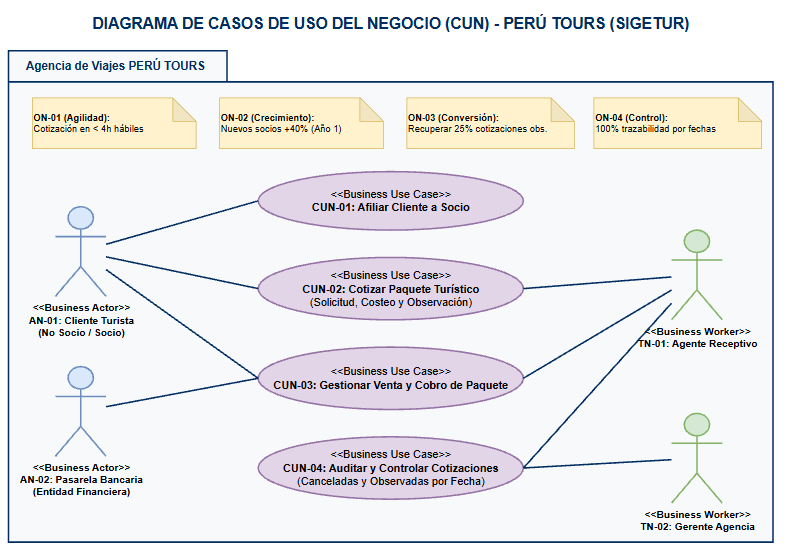
\includegraphics[width=0.80\textwidth]{../diagramas/diagram_cun.png}
\end{frame}

% ----------------- SLIDE 11: DIAGRAMA DE ACTIVIDADES (SWIMLANES) -----------------
\begin{frame}{Diagrama de Actividades con Carriles (Swimlanes)}
    \centering
    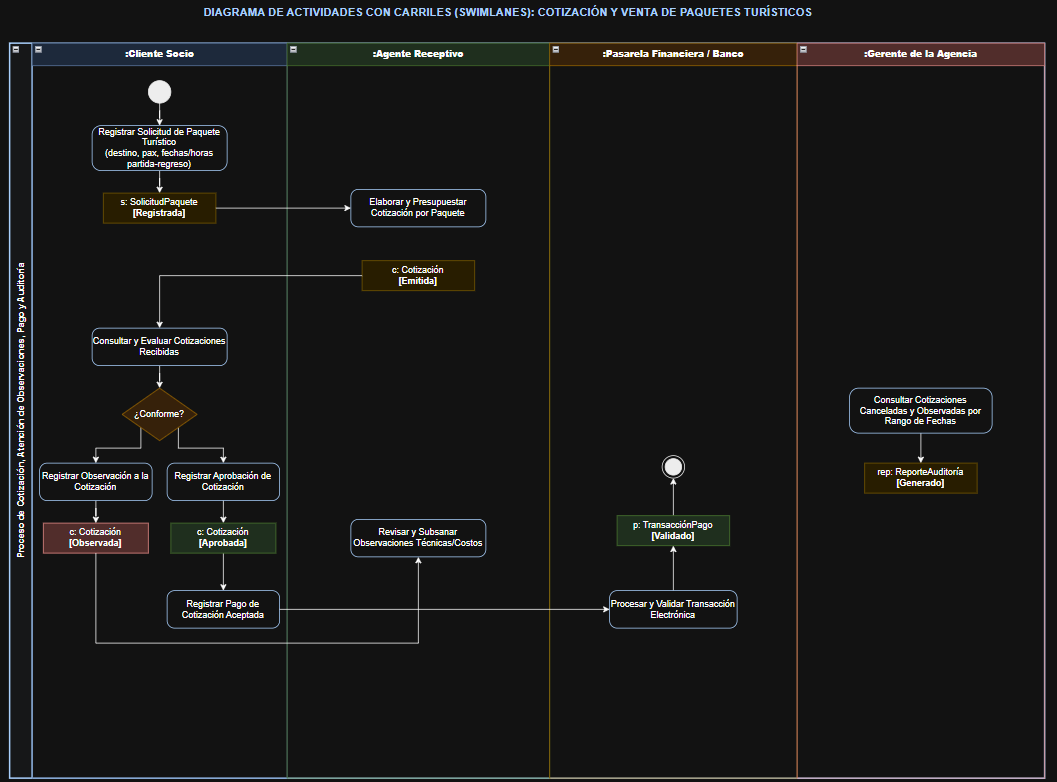
\includegraphics[width=0.78\textwidth]{../diagramas/diagram_actividades.png}
\end{frame}

% ----------------- SLIDE 12: OBJETOS DEL NEGOCIO Y CICLO DE ESTADOS -----------------
\begin{frame}{Ciclo de Vida y Estados de los Objetos del Negocio}
    \small
    El flujo de datos entre actividades produce y transforma entidades clave del negocio:
    \vspace{0.2cm}
    \begin{block}{\textbf{Máquina de Estados de la Cotización (\texttt{c: Cotización})}}
        \centering
        \texttt{[Emitida]} $\longrightarrow$ \texttt{[Observada]} $\rightleftharpoons$ \texttt{[Reajustada]}\\[0.15cm]
        $\downarrow$\\[0.15cm]
        \texttt{[Aprobada]} $\longrightarrow$ \texttt{[Pagada / Formalizada]}\\[0.15cm]
        \textit{(o bien)} $\longrightarrow$ \texttt{[Cancelada / Expirada]}
    \end{block}
    \vspace{0.2cm}
    \begin{columns}[t]
        \begin{column}{0.48\textwidth}
            \begin{exampleblock}{\textbf{Objeto SolicitudPaquete}}
                \footnotesize
                $\bullet$ \texttt{[Registrada]} $\rightarrow$ \texttt{[Asignada]} $\rightarrow$ \texttt{[Atendida]}.
            \end{exampleblock}
        \end{column}
        \begin{column}{0.48\textwidth}
            \begin{exampleblock}{\textbf{Objeto TransacciónPago}}
                \footnotesize
                $\bullet$ \texttt{[Pendiente]} $\rightarrow$ \texttt{[Procesado]} $\rightarrow$ \texttt{[Validado]}.
            \end{exampleblock}
        \end{column}
    \end{columns}
\end{frame}

% ----------------- SLIDE 13: REQUISITOS FUNCIONALES (RF01 - RF08) -----------------
\begin{frame}{Especificación de Requisitos Funcionales (RF)}
    \scriptsize
    \begin{table}[H]
    \centering
    \begin{tabularx}{\textwidth}{|c|l|X|c|}
    \hline
    \textbf{Código} & \textbf{Requisito Funcional} & \textbf{Descripción Técnica} & \textbf{Rol} \\ \hline
    \textbf{RF01} & Afiliación de Clientes & Registro de clientes no socios mediante formulario web validado. & No Socio \\ \hline
    \textbf{RF02} & Registro de Solicitudes & Captura de destino, n° personas, fechas y horas de partida y regreso. & Socio \\ \hline
    \textbf{RF03} & Emisión de Cotizaciones & Presupuestación de servicios y fijación de costos por el agente receptivo. & Agente \\ \hline
    \textbf{RF04} & Consulta de Cotizaciones & Listado interactivo y comparativa de cotizaciones recibidas. & Socio \\ \hline
    \textbf{RF05} & Aprobación de Cotización & Registro de aceptación formal de una cotización y habilitación de pago. & Socio \\ \hline
    \textbf{RF06} & Registro de Observaciones & Ingreso de observaciones técnicas o económicas a cotizaciones de interés. & Socio \\ \hline
    \textbf{RF07} & Registro de Pago & Abono mediante pasarela segura y emisión de constancia digital. & Socio \\ \hline
    \textbf{RF08} & Consulta de Auditoría & Filtrado de cotizaciones canceladas u observadas por rango de fechas. & Gerente / Agente \\ \hline
    \end{tabularx}
    \end{table}
\end{frame}

% ----------------- SLIDE 14: REQUISITOS NO FUNCIONALES Y REGLAS DE NEGOCIO -----------------
\begin{frame}{Requisitos No Funcionales (FURPS+) y Reglas de Negocio}
    \begin{columns}[t]
        \begin{column}{0.48\textwidth}
            \begin{block}{\textbf{Requisitos No Funcionales (FURPS+)~\cite{pressman2015}}} % Cita: Modelo FURPS+ (Pressman & Maxim)
                \scriptsize
                \begin{itemize}
                    \item \textbf{Usabilidad:} 100\% responsive en web y móvil; flujo en $< 4$ clics.
                    \item \textbf{Rendimiento:} Consultas y reportes con latencia $< 1.8$ segundos.
                    \item \textbf{Seguridad:} Autenticación RBAC, cifrado HTTPS TLS 1.3 y hash Argon2id.
                    \item \textbf{Disponibilidad:} Uptime de servidores $\ge 99.5\%$.
                \end{itemize}
            \end{block}
        \end{column}
        \begin{column}{0.48\textwidth}
            \begin{alertblock}{\textbf{Reglas del Negocio (RN)}}
                \scriptsize
                \begin{itemize}
                    \item \textbf{RN01:} Solo socios activos pueden solicitar y consultar cotizaciones.
                    \item \textbf{RN02:} Fecha/hora de regreso estrictamente posterior a la de partida.
                    \item \textbf{RN03:} Solo cotizaciones \textbf{[Aprobadas]} pueden recibir pago.
                    \item \textbf{RN04:} Cotizaciones observadas requieren reajuste antes de aprobarse.
                    \item \textbf{RN05:} Auditoría reservada a Agente y Gerente.
                \end{itemize}
            \end{alertblock}
        \end{column}
    \end{columns}
\end{frame}

% ----------------- SLIDE 15: TRAZABILIDAD Y CONCLUSIONES -----------------
\begin{frame}{Matriz de Trazabilidad y Siguiente Fase (Semana 5)}
    \begin{columns}[t]
        \begin{column}{0.52\textwidth}
            \begin{block}{\textbf{Matriz de Trazabilidad Integral}}
                \scriptsize
                \begin{tabular}{|c|c|c|}
                \hline
                \textbf{Objetivo} & \textbf{CUN} & \textbf{Requisitos (RF)} \\ \hline
                ON-02 & CUN-01 Afiliación & RF01 \\ \hline
                ON-01 & CUN-02 Cotización & RF02, RF03, RF04, RF05 \\ \hline
                ON-03 & CUN-02 Cotización & RF06 (Observaciones) \\ \hline
                ON-01 & CUN-03 Venta/Pago & RF07 (Pasarela) \\ \hline
                ON-04 & CUN-04 Auditoría & RF08 (Filtro Fechas) \\ \hline
                \end{tabular}
            \end{block}
        \end{column}
        \begin{column}{0.45\textwidth}
            \begin{exampleblock}{\textbf{Conexión a Semana 5 (Elaboración)}}
                \small
                \begin{itemize}
                    \item Definición de Casos de Uso del Sistema (CUS).
                    \item Especificación detallada de casos de uso (CUS).
                    \item Diseño de prototipos GUI en Figma.
                    \item Diagramas de Clases del Dominio y Clases de Análisis.
                \end{itemize}
            \end{exampleblock}
        \end{column}
    \end{columns}
\end{frame}

% ----------------- SLIDE 16: REFERENCIAS BIBLIOGRÁFICAS -----------------
\begin{frame}{Referencias Bibliográficas}
    \footnotesize
    \begin{thebibliography}{9}
        \bibitem{garciamolina} García Molina, J. et al. (2000). De los Procesos del Negocio a los Casos de Uso. Univ. de Murcia.
        \bibitem{rup2000} Jacobson, I., Booch, G., \& Rumbaugh, J. (2000). El Proceso Unificado de Desarrollo de Software. Addison-Wesley.
        \bibitem{swebok2024} IEEE Computer Society (2024). SWEBOK v4: Guide to the Software Engineering Body of Knowledge.
        \bibitem{pressman2015} Pressman, R. \& Maxim, B. (2015). Ingeniería del Software: Un enfoque práctico. McGraw-Hill.
        \bibitem{mincetur2020} MINCETUR (2020). Reglamento de Agencias de Viajes y Turismo, D.S. N° 005-2020-MINCETUR.
    \end{thebibliography}
\end{frame}

% ----------------- SLIDE 17: PREGUNTAS Y CIERRE -----------------
\begin{frame}
    \centering
    \vspace{1cm}
    {\huge \textbf{¡Muchas Gracias!}}\\[0.6cm]
\end{frame}

\end{document}
